\documentclass[10pt,aspectratio=43,mathserif]{beamer}		
%设置为 Beamer 文档类型,设置字体为 10pt,长宽比为16:9,数学字体为 serif 风格

%%%%-----导入宏包-----%%%%
\usepackage{seu}
\usepackage{xeCJK}
\usepackage{amsmath,amsfonts,amssymb,bm}
\usepackage{color}
\usepackage{graphicx,hyperref,url}
\usepackage{booktabs}
\renewcommand{\thempfootnote}{\arabic{mpfootnote}}
%%%%%%%%%%%%%%%%%%


%%%%-----设置字体-----%%%%
%Windows和Mac OS下都可用
\setsansfont[Path=fonts/]{Helvetica}

%\setsansfont{Times New Roman}

%仅Windows可用
%\setCJKmainfont{Hiragino Sans GB W3}

%仅Mac OS下可用
%\setCJKmainfont{Songti SC}




%设置 Beamer 主题
\beamertemplateballitem


\AtBeginSection[]
{
  \begin{frame}<beamer>
    \frametitle{\textbf{目录}}
    \textbf{\tableofcontents[currentsection]}
  \end{frame}
}

%%%%----首页信息设置----%%%%
%%%%----标题设置
\title[高光谱图像的非凸低秩表示]{
	\fontsize{14pt}{25pt}\selectfont \textbf{高光谱图像的非凸低秩表示}
}
\subtitle{\fontsize{13pt}{14pt}\selectfont {在图像降噪方面的使用}}			
%%%%----机构信息
\institute[SEU]{
	\fontsize{11pt}{12pt}\selectfont {东南大学{\quad}吴健雄学院}
}
%%%%----个人信息设置
\author[陈安皓]{
	学生姓名:陈安皓\\
	指导教师:贾育衡
}
%%%%----日期信息
\date[2021年6月8日]{
 2021年6月8日
}

\begin{document}
%生成标题页
\begin{frame}
\titlepage
\end{frame}

\section*{目录}

\begin{frame}
\frametitle{\textbf{目录}}
\textbf{\tableofcontents}
\end{frame}

\section[引言]{引言}

\begin{frame}
\frametitle{\textbf{背景知识}}
\begin{block}{\textbf{高光谱图像及其成像原理}}
% 插入图片
\begin{figure}[H]
\centering
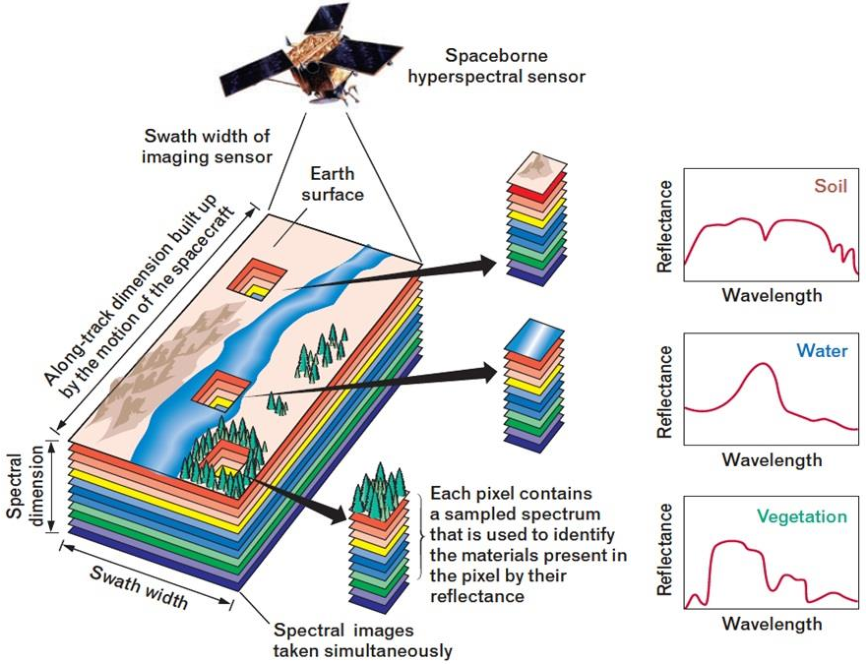
\includegraphics[scale=0.22]{img-principleofphotograph.png}
\caption{高光谱图像的成像原理\footnote{图片来源:semanticscholar.org}}
\end{figure}
\end{block}
\end{frame}
    
\begin{frame}
\frametitle{\textbf{背景知识}}
\begin{block}{\textbf{高光谱图像的特征}}
% 插入图片
\begin{figure}[H]
\centering
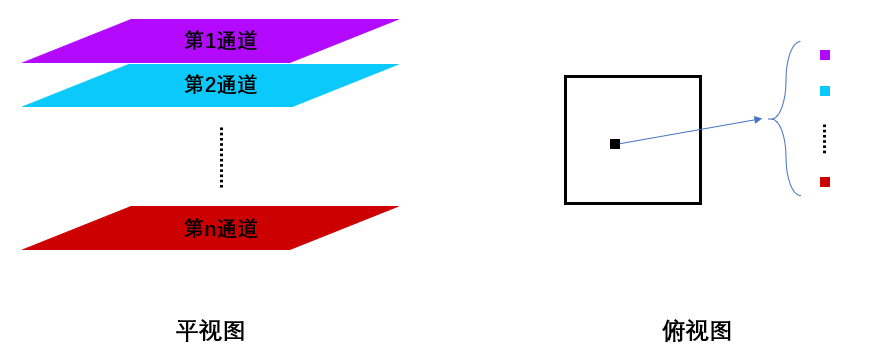
\includegraphics[scale=0.5]{img-characterofphotograph.png}
\caption{高光谱图像的特征}
\end{figure}
\end{block}
    	
\begin{block}{\textbf{高光谱图像的部分应用领域}}
$\bullet$农业 \qquad 
$\bullet$军事 \qquad 
$\bullet$环境 \qquad 
$\bullet$地学
\end{block}
\end{frame}

\section[相关工作]{相关工作}
\begin{frame}
\frametitle{\textbf{相关工作}}
	
\end{frame}

\section[研究路线]{研究路线}
\begin{frame}
\frametitle{\textbf{问题建模}}
\par 假设一幅一维图像$Y$受到噪声的污染,即:
\begin{displaymath}
Y = X + N
\end{displaymath}
式中,
\par$X$代表未受到污染的、干净的图像,大小为$m \times n$;
\par$N$代表噪声,大小为$m \times n$;
\par$Y$代表成像设备获取到的图像,即受到污染的图像,大小为$m \times n$。
\newline
\par 那么,图像降噪的工作就是将$Y$复原为$X$。
\end{frame}

\begin{frame}
\frametitle{\textbf{问题建模}}
\begin{block}{\textbf{自然图像的低秩性}}
\begin{columns}
\column{.5\textwidth}
\begin{figure}[!t]
\centering
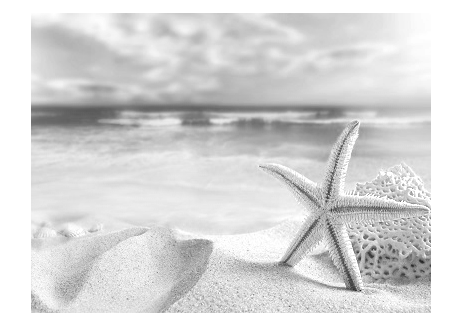
\includegraphics[scale=0.3]{example-figure.png}
\caption{一张自然图像}
\label{example-figure}
\end{figure}

\column{.5\textwidth}
\begin{figure}[!t]
\centering
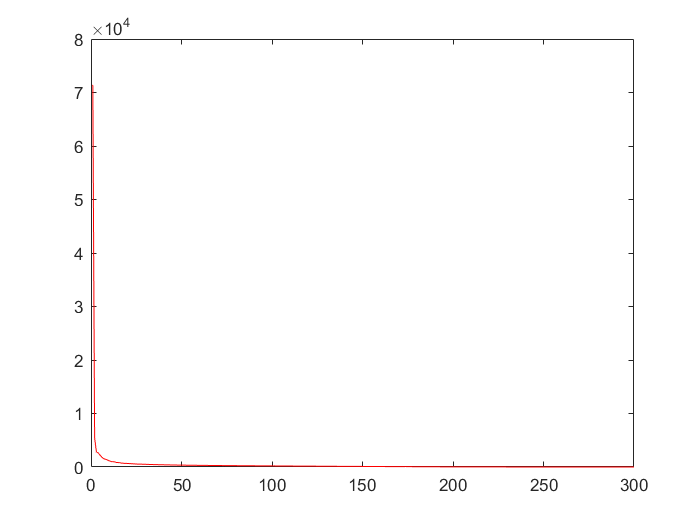
\includegraphics[scale=0.2]{example-figure-svd.png}
\caption{图\ref{example-figure}的奇异值分布图}
\label{example-figure-svd}
\end{figure}
\end{columns}
\end{block}
\par 基于低秩假设的图像降噪方法可以被形式化为
\begin{displaymath}
arg\min\limits_{X} \quad rank(X)
\end{displaymath}
\end{frame}

\begin{frame}
\frametitle{\textbf{问题建模}}
\par 在对图像进行降噪处理时,既需要去除图像里的噪声,同时也需要尽可能地保留原来的信息。因此,实际上,需要求解的最优化问题是
\begin{equation}
\centering
arg\min\limits_{X} \quad \left\|Y-X\right\|_F^2 + \lambda \cdot rank(X)
\label{F-rank}
\end{equation}
式中,
\par$X$代表未受到污染的、干净的图像,大小为$m \times n$;
\par$N$代表噪声,大小为$m \times n$;
\par$Y$代表成像设备获取到的图像,即受到污染的图像,大小为$m \times n$;
\par$\left\|*\right\|_F$表示$Frobenius$范数;
\par$\lambda$是正则化参数。

\end{frame}

\begin{frame}
\frametitle{\textbf{用(普通)核范数替代秩函数}}
\par 然而,式\ref{F-rank}
\begin{displaymath}
arg\min\limits_{X} \quad \left\|Y-X\right\|_F^2 + \lambda \cdot {\color{red}{rank(X)}}
\end{displaymath}
\par 是一个NP-hard问题。
\newline
\newline
\par 通常使用秩函数的凸近似,也就是核范数,作为式\ref{F-rank}中秩函数的替代:
\begin{equation}
\centering
arg\min\limits_{X} \quad \left\|Y-X\right\|_F^2 + \lambda \cdot {\color{red}{\left\|X\right\|_*}}
\label{F-NN}
\end{equation}
式中,
\par $\left\|*\right\|_*$表示核范数。
\par $\left\|X\right\|_* = \sum\limits_{i=1}^{n}\sigma_i(X)$,$\sigma_i(X)$表示矩阵$X$的第$i$个奇异值。
\end{frame}

\begin{frame}
\frametitle{\textbf{用截断式核范数替代秩函数}}
\begin{columns}
\column{.55\textwidth}
\par 式\ref{F-rank}
\begin{displaymath}
	arg\min\limits_{X} \quad \left\|Y-X\right\|_F^2 + \lambda \cdot {\color{red}{rank(X)}}
\end{displaymath}
\par 更新为
\begin{equation}
	\centering
	arg\min\limits_{X} \quad \left\|Y-X\right\|_F^2 + \lambda \cdot {\color{red}{\left\|X\right\|_{tr,*}}}
	\label{F-TNN}
\end{equation}
式中,
\par $\left\|*\right\|_{tr,*}$表示截断式核范数。
\par $\left\|X\right\|_{tr,*} = \sum\limits_{i=r+1}^{n}\sigma_i(X)$

\column{.45\textwidth}
\begin{figure}[!t]
\centering
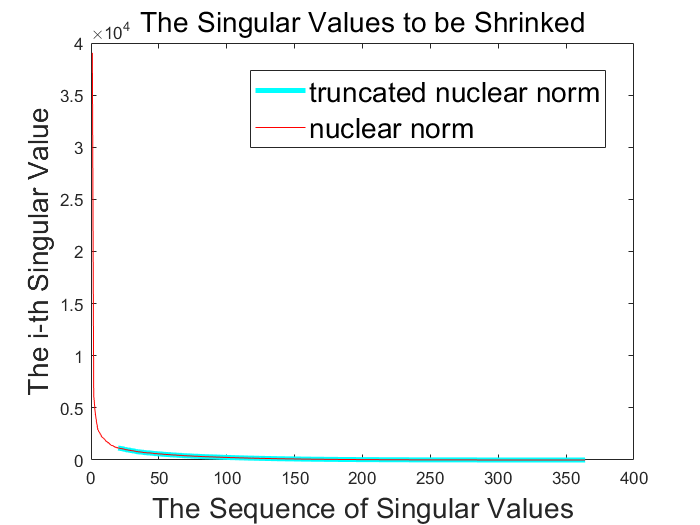
\includegraphics[scale=0.3]{surrogate-to-rank-2.png}
\caption{截断式核范数的几何意义(取$r=19$)}
\label{surrogate-to-rank-2}
\end{figure}
\end{columns}
\end{frame}

\begin{frame}
\frametitle{\textbf{用权重式核范数替代秩函数}}
\par 式\ref{F-rank}
\begin{displaymath}
arg\min\limits_{X} \quad \left\|Y-X\right\|_F^2 + \lambda \cdot {\color{red}{rank(X)}}
\end{displaymath}
\par 更新为
\begin{equation}
\centering
arg\min\limits_{X} \quad \left\|Y-X\right\|_F^2 + \lambda \cdot {\color{red}{\left\|X\right\|_{w,*}}}
\label{F-WNN}
\end{equation}
式中,
\par $\left\|*\right\|_{w,*}$表示权重式核范数。
\par $\left\|X\right\|_{w,*} = \sum\limits_{i=1}^{n}w_i\sigma_i(X)$
	
\end{frame}

\begin{frame}
\frametitle{\textbf{用$log$-核范数替代秩函数}}
\begin{columns}
	\column{.55\textwidth}
	\par 式\ref{F-rank}
	\begin{displaymath}
		arg\min\limits_{X} \quad \left\|Y-X\right\|_F^2 + \lambda \cdot {\color{red}{rank(X)}}
	\end{displaymath}
	\par 更新为
	\begin{equation}
		\centering
		arg\min\limits_{X} \quad \left\|Y-X\right\|_F^2 + \lambda \cdot {\color{red}{\left\|X\right\|_{log,*}}}
		\label{F-LNN}
	\end{equation}
	式中,
	\par $\left\|*\right\|_{log,*}$表示$log$-核范数。
	\par $\left\|X\right\|_{log,*} = \sum\limits_{i=1}^{n}log(\sigma_i(X)+1)$
	
	\column{.45\textwidth}
	\begin{figure}[!t]
		\centering
		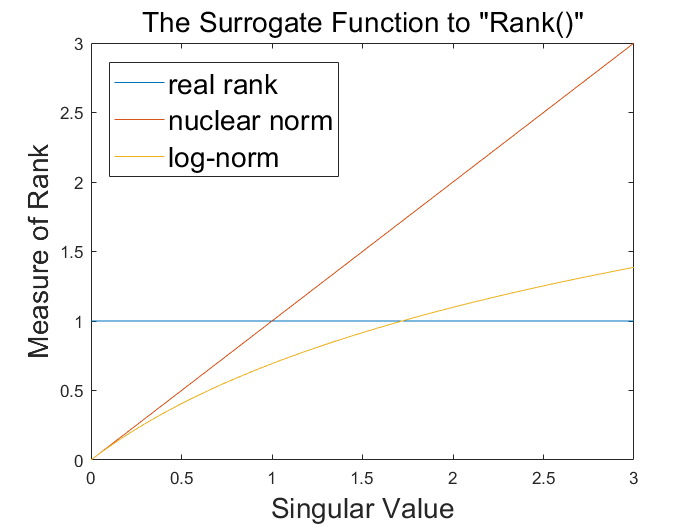
\includegraphics[scale=0.3]{surrogate-to-rank-1.png}
		\caption{$log$-核范数的几何意义}
		\label{surrogate-to-rank-1}
	\end{figure}
\end{columns}
\end{frame}

%\section[方法]{研究方法与数据集特征}
%
%
%		\begin{frame}
%		  \frametitle{\textbf{爬取公共短消息网关}}
%            % ----------------分栏的结构开始---------------- %
%            % 该结构中使用block分开两个内容区
%            % 可根据需要进行图文混排?我还没试过,我想应该可以
%            \begin{columns}
%                \column{.5\textwidth}
%                \footnotesize
%                \begin{itemize}
%                  \item 使用Scrapy框架爬取公共网关
%                  \item 收集8个公共短信网关在14个月的数据
%                  \item 共抓取386,327条数据
%                \end{itemize}
%
%                \column{.5\textwidth}
%                \begin{table}
%                \caption{公共网关及抓取的信息数}
%                \label{table1:gateways}
%                \centering
%                \footnotesize
%                \begin{tabular}{|c|c|}
%                \hline
%                \textbf{Site}           & \textbf{Messages}\\
%                \hline
%                receivesmsonline.net    &81313\\
%                \hline
%                receive-sms-online.info &69389\\
%                \hline
%                receive-sms-now.com     &63797\\
%                \hline
%                 hs3x.com               &55499\\
%                \hline
%                receivesmsonline.com    &44640\\
%                \hline
%                receivefreesms.com      &37485\\
%                \hline
%                receive-sms-online.com  &27094\\
%                \hline
%                 e-receivesms.com       &7107\\
%                \hline
%                \end{tabular}
%                \end{table}
%            \end{columns}
%
%		\end{frame}
%
%        \begin{frame}
%		  \frametitle{\textbf{消息聚类分析}}
%            \begin{block}{\textbf{基本思路}}
%                \begin{itemize}
%                    \item 使用编辑距离矩阵将类似的消息归于一张连通图中。
%                    \item 使用固定值替换感兴趣的消息,如代码、email地址。
%                    \item 查找归一化距离小于阈值的消息,并确定聚类边界。
%                \end{itemize}
%            \end{block}
%
%            \begin{block}{\textbf{实现步骤}}
%                \begin{enumerate}
%                  \item 加载所有消息。
%                  \item 用固定的字符串替换数字、电子邮件和URL以预处理消息。
%                  \item 将预处理后的信息按字母排序。
%                  \item 通过使用编辑距离阈值(0.9)来确定聚类边界。
%                  \item 手动标记各个聚类,以确定服务提供者、消息类别等。
%                \end{enumerate}
%            \end{block}
%		\end{frame}
%
%        \begin{frame}
%		  \frametitle{\textbf{消息分类结果}}
%            \begin{itemize}
%                \item \textbf{账户创建确认信息}:向来自服务提供者的用户提供了一个代码,该服务提供者需要在新帐户创建期间进行SMS验证。
%                \item \textbf{活动确认信息}:向来自服务提供者的用户提供了请求授权进行活动的代码(例如,付款确认)。
%                \item \textbf{一次性密码}:包含用户登录的代码的短信息。
%                \item \textbf{用于绑定不同设备的一次性口令}:将消息发送给用户,以绑定一个新的电话号码或启用相应的移动应用程序。
%                \item \textbf{重置密码口令}:包含密码重置密码的短信息。
%                \item \textbf{其他}:其他未被指定为某种特定功能的消息。
%            \end{itemize}
%		\end{frame}
%
%        \begin{frame}
%		  \frametitle{\textbf{消息分类结果}}
%            \begin{columns}
%                \column{.5\textwidth}
%                \footnotesize
%                \begin{itemize}
%                  \item 账户创建和移动设备绑定占比最大,占51.6\%
%                  \item 一次性密码信息占7.6\%
%                  \item 密码重置消息占1.3\%
%                  \item 包含“测试”关键词的消息占0.8\%
%                \end{itemize}
%
%                \column{.5\textwidth}
%                \begin{figure}[!t]
%                    \centering
%                    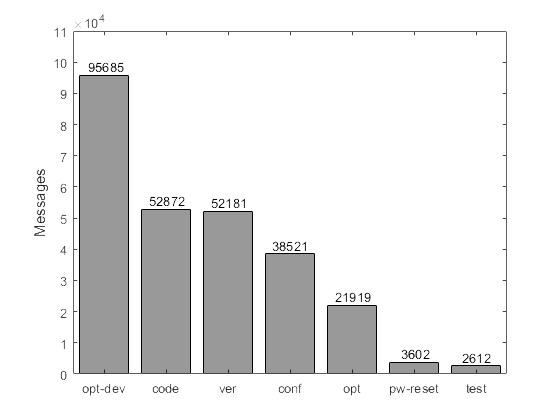
\includegraphics[width=1.1\textwidth]{figures/figure4.png}
%                    \caption{消息的聚类}
%                    \label{figure3_OTT}
%                \end{figure}
%            \end{columns}
%		\end{frame}
%
%
%
%\section[分析]{SMS使用情况分析}
%
%
%		\begin{frame}
%		  \frametitle{\textbf{使用SMS作为安全信道}}
%		  \begin{block}{\textbf{PII和其他敏感信息}}
%                \begin{itemize}
%                    \item 财务信息
%                    \item 用户名和密码
%                    \item 重置密码口令
%                    \item 其他个人识别信息(PII)
%                    \item 敏感程序的SMS活动
%                \end{itemize}
%            \end{block}
%		\end{frame}
%
%        \begin{frame}
%		  \frametitle{\textbf{使用SMS作为安全信道}}
%            \begin{block}{\textbf{SMS编码熵}}
%                使用 $\chi$方检验测试每组编码的熵。$\chi$方检验是一个零假设的显著性检验,用于测试SMS服务的编码是否是从低位到高位均匀分布的。若p值小于0.01,则表明观测值和理想均匀分布之间存在统计学上的显著差异。
%                检验结果表明,65\%的SMS服务的编码熵较低,容易被预测和攻击。
%            \end{block}
%            \begin{columns}
%
%                \column{.26\textwidth}
%                \begin{figure}
%                    \centering
%                    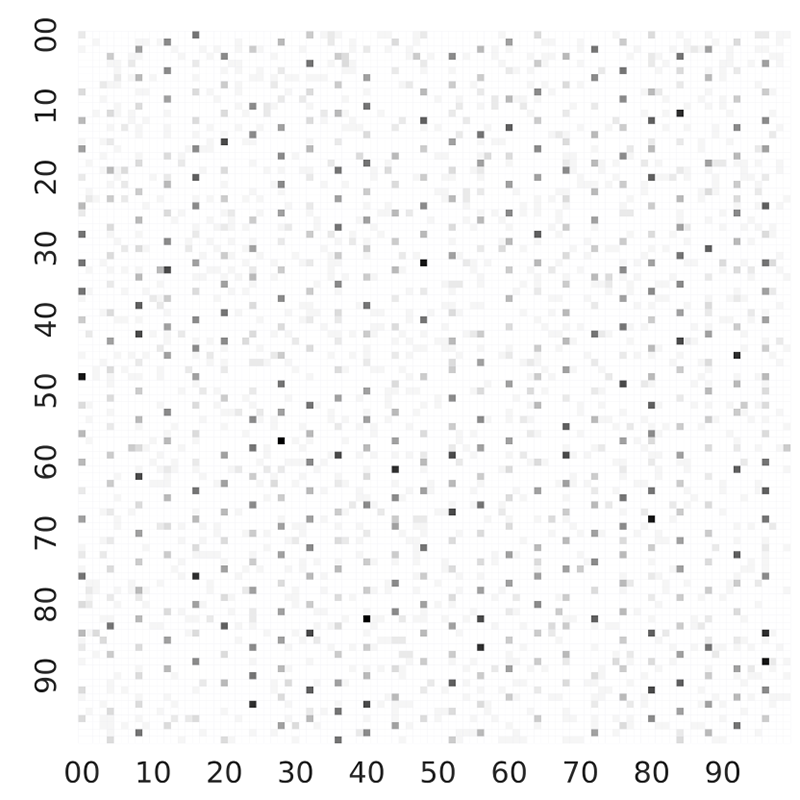
\includegraphics[width=1.1\textwidth]{figures/figure6.png}
%                    \caption{WeChat}
%                    \label{figure6_WeChat}
%                \end{figure}
%
%                \column{.26\textwidth}
%                \begin{figure}
%                    \centering
%                    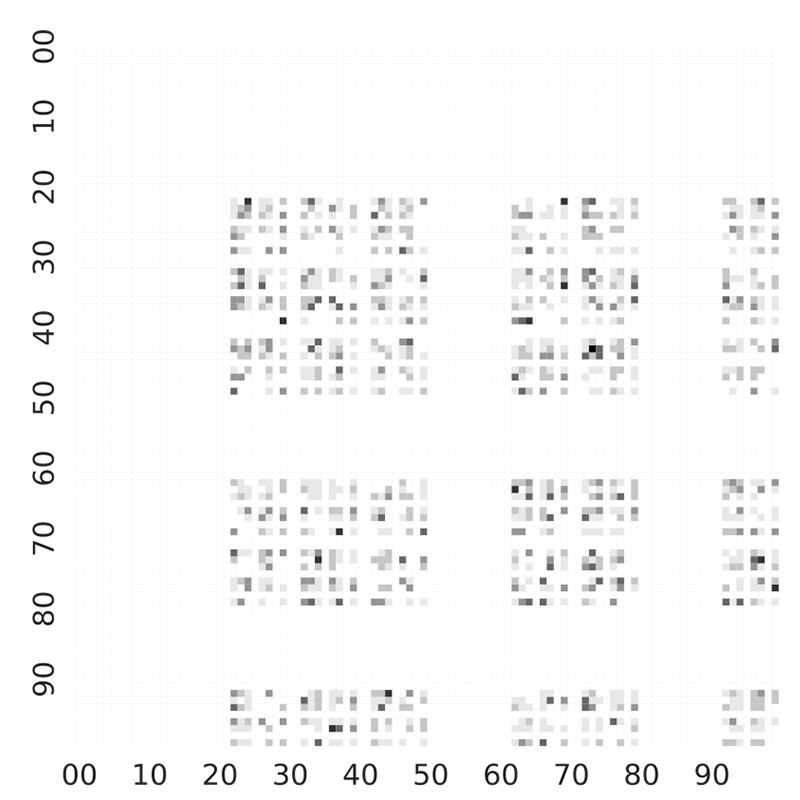
\includegraphics[width=1.1\textwidth]{figures/figure7.png}
%                    \caption{Talk2}
%                    \label{figure3_Talk2}
%                \end{figure}
%
%                \column{.26\textwidth}
%                \begin{figure}
%                    \centering
%                    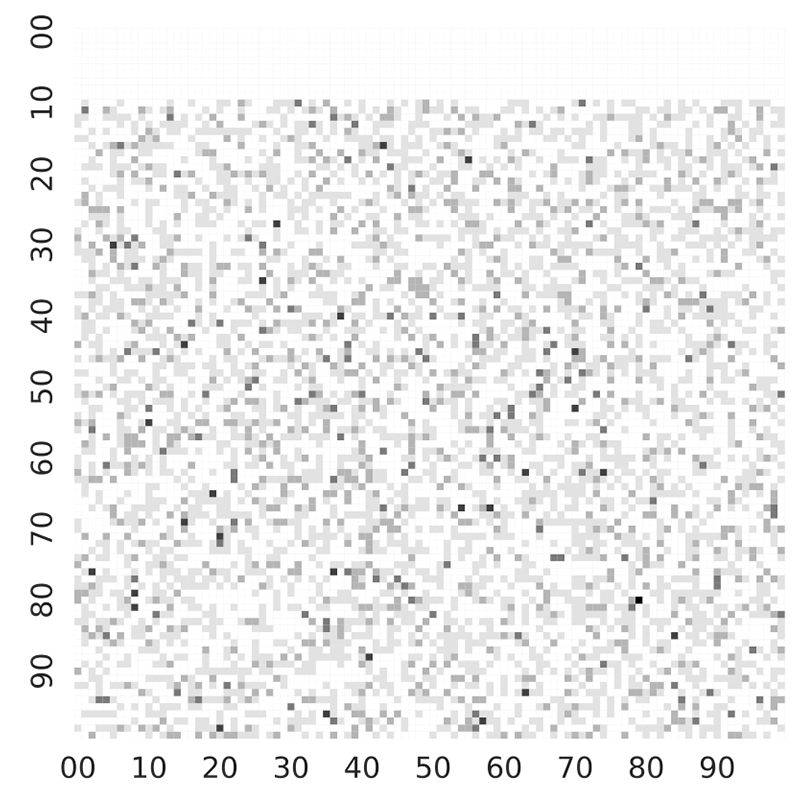
\includegraphics[width=1.1\textwidth]{figures/figure8.png}
%                    \caption{Google}
%                    \label{figure3_Google}
%                \end{figure}
%
%            \end{columns}
%
%		\end{frame}
%
%		\begin{frame}
%		  \frametitle{\textbf{SMS的恶意应用}}
%            \begin{block}{\textbf{公共网关检测到的恶意信息}}
%    		  \begin{itemize}
%    		    \item \textbf{泄露用户位置信息}:短URL可以用于确定消息的源和目的地,即会泄漏用户的位置信息。
%    		    \item \textbf{垃圾邮件宣传广告}:在公共网关服务中比例较低,约为1.0\%。
%                \item \textbf{网络钓鱼活动}:试图欺骗用户,使其相信自己正与合法网站通信。
%    		  \end{itemize}
%            \end{block}
%
%            \begin{columns}
%
%                \column{.26\textwidth}
%                \begin{figure}
%                    \centering
%                    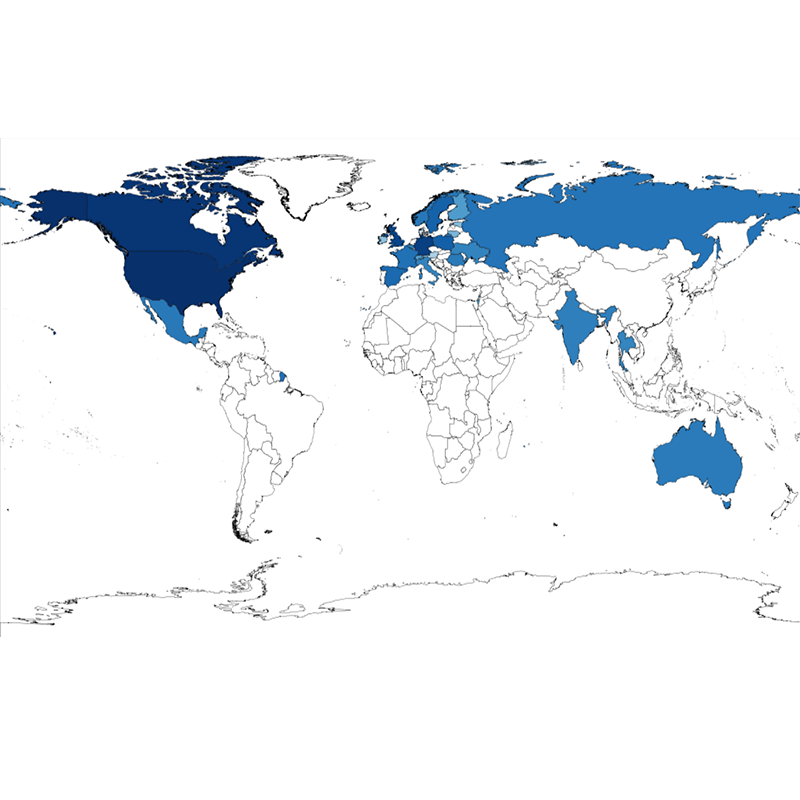
\includegraphics[width=1.1\textwidth]{figures/figure9.png}
%                    \caption{SMS地址分布}
%                    \label{figure9_WeChat}
%                \end{figure}
%
%                \column{.26\textwidth}
%                \begin{figure}
%                    \centering
%                    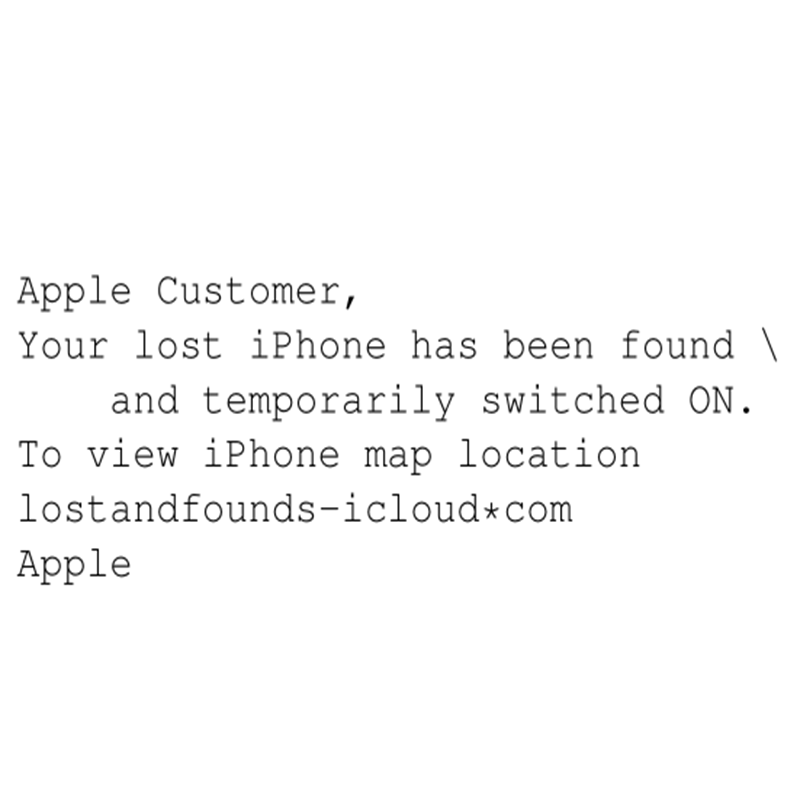
\includegraphics[width=1.1\textwidth]{figures/figure10.png}
%                    \caption{钓鱼短信实例}
%                    \label{figure10_Talk2}
%                \end{figure}
%
%                \column{.26\textwidth}
%                \begin{figure}
%                    \centering
%                    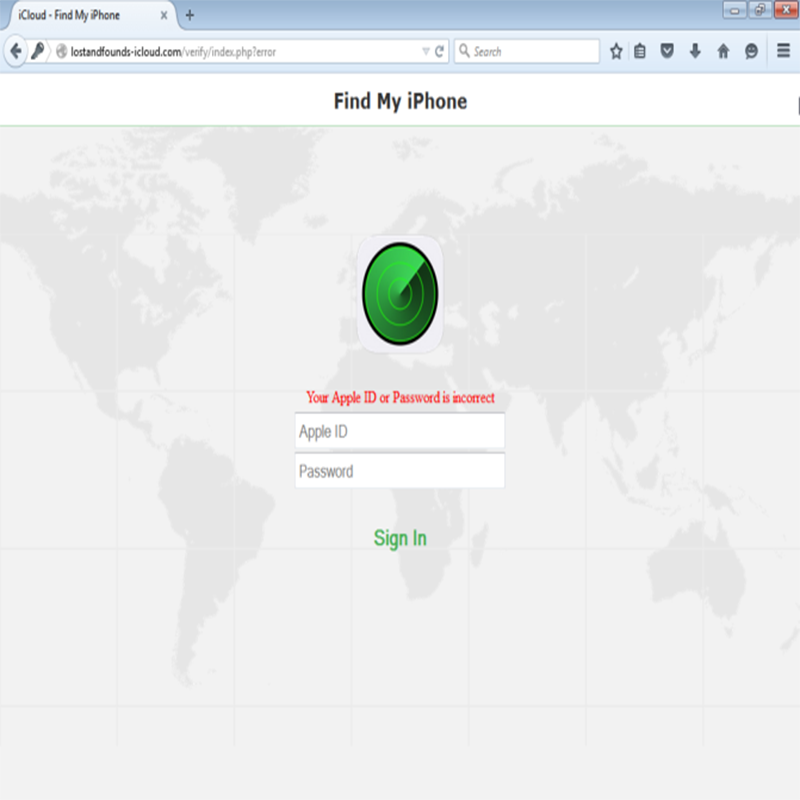
\includegraphics[width=1.1\textwidth]{figures/figure11.png}
%                    \caption{钓鱼网站}
%                    \label{figure11_Talk2}
%                \end{figure}
%
%            \end{columns}
%
%		\end{frame}
%
%\section[结论]{结论}
%
%
%		\begin{frame}
%		  \frametitle{\textbf{结论}}
%		
%		  \begin{itemize}
%		    \item SMS生态系统在智能手机时代出现了新的发展,加入了更多新的设备和参与者。
%		    \item 公共网关为用户提供了基于SMS的各种安全解决方案。
%            \item 根据该研究,将SMS作为安全信道传递敏感信息存在一定的危险性。一些一次性的消息传递机制亟待改进。
%            \item 至于短信滥用,公共网关可以用于规避一些安全性较差的认证机制,或进行PVA欺诈行为。
%		  \end{itemize}
%		\end{frame}
%
%
%\section*{}
%            \begin{frame}
%
%                \begin{center}
%                    \begin{minipage}{1\textwidth}
%                        \setbeamercolor{mybox}{fg=white, bg=black!60!green}
%                        \begin{beamercolorbox}[wd=0.70\textwidth, rounded=true, shadow=true]{mybox}
%                        \LARGE \centering Thanks for Listening.
%                        \end{beamercolorbox}
%                    \end{minipage}
%                \end{center}
%
%                \begin{figure}[!t]
%                    \centering
%                    
\includegraphics[width=.8\textwidth]{figures/figure5.png}
%                    \label{figure4_ad}
%                \end{figure}
%            \end{frame}
\section[总结]{总结}
%\begin{frame}
%\frametitle{\textbf{总结}}
%	
%\end{frame}
\section[QA]{Q\&A}
%\begin{frame}
%\frametitle{\textbf{Q\&A}}
%	
%\end{frame}
\section*{}
\begin{frame}
\begin{center}
\begin{minipage}{1\textwidth}
\setbeamercolor{mybox}{fg=white, bg=black!60!green}
\begin{beamercolorbox}[wd=0.70\textwidth, rounded=true, shadow=true]{mybox}
\LARGE \centering 感谢各位评委老师们的聆听!
\end{beamercolorbox}
\end{minipage}
\end{center}
\end{frame}
\end{document}
